\section{Durchführung als Projekt}
\subsection{Ziele}
\steffen
Ziel der Unterrichtsreihe ist es, die Schüler den mathematischen Modellierungskreislauf herleiten und durchführen zu lassen. Als Modellierungsobjekt dient dabei die Modellierung von Epidemien und Pandemien. 


\begin{landscape}
\subsection{Reihenplanung}
\noindent
\begin{longtable}{|C{0.05\textwidth}|L{0.2\textwidth}|L{0.3\textwidth}|L{0.25\textwidth}|L{0.3\textwidth}|L{0.25\textwidth}|L{0.1\textwidth}|}
\hline
Std&Inhalte&Grobziele \& Kompetenzen&Wdh \& Festigung&didakt. \& method. Auswahl&Medien&Sonstiges\\
\hline\hline
\endhead
\hline
\endfoot
1\&{}2 &\emph{SIHDR}&\begin{itemize}
	\item Schüler durchlaufen den Modellierungskreislauf zwei mal
	\item K2
	\item K3
\end{itemize}&--&\begin{itemize}
	\item Modell von \emph{SID} zu \emph{SIHDR}
	\item TPS zur Modellbildung
	\item Zwischenergebnisse werden in der Klasse besprochen
	\item Durch Aufgabenstellung wenig Varianz in Modellierung
\end{itemize}&\begin{itemize}
	\item Ta\-bel\-len\-kal\-ku\-la\-tion
\end{itemize}&--\\\hline
3\&{}4&\begin{itemize}
	\item Mo\-del\-lier\-ungs\-kreis\-lauf
	\item \emph{SIHFDR}
\end{itemize}&b&c&d&e&f\\\hline
5\&{}6&\begin{itemize}
	\item Maß\-nahmen gegen Ausbreitung
	\item Schwächen des Modells
	\item Erwei\-terung auf mehrere Nationen
\end{itemize}&\begin{itemize}
	\item K2
	\item K3
\end{itemize}&Model der Vorstunde&d&e&f\\
\end{longtable}
\end{landscape}
\subsection{Projektstunde 1 \& 2}\ellen
\subsubsection{Bemerkungen zur Lerngruppe}
Bei der Planung der ersten beiden Stunden war uns lediglich bekannt, dass es sich um Schülerinnen und Schüler der zehnten Klasse eines Gymnasiums für Hochbegabte handelt\\
Zudem seien die Grundlagen der Schülerinnen und Schüler höchst unterschiedlich. Der Umgang mit Tabellenkalkulationsprogrammen sollte jedoch in Grundzügen beherrscht werden. 
\subsubsection{Methodische Überlegungen}
Um die Motivation zu fördern und eine möglichst hohe Nachhaltigkeit zu erhalten, sollen die Unterrichtsstunden handlungsorientiert ausgerichtet werden. Dazu sollen die Schülerinnen und Schüler zunächst alleine Rechenoperationen formulieren, mit deren Hilfe die Größe der Klassen (Gesund, Krank und Tod) berechnet werden können.\\
Die Schülerinnen und Schüler haben bereits vorher im Mathematikunterricht gelernt, wie sie aus Texten Terme aufstellt. Dadurch können die Schülerinnen und Schüler früh Erfolge erringen um dadurch die Motivation zu behalten und um ihnen die Angst vor dem Simulieren nehmen.\\
Durch die Einzelarbeit ist gewährleistet, dass alle Schülerinnen und Schüler sich am Unterricht beteiligen. Sobald alle Schülerinnen und Schüler ihre Terme aufgestellt haben, vergleichen sie ihre mit denen ihres Nachbarn.\\
Dadurch können die Schülerinnen und Schüler mathematisches argumentieren einüben. Zusätzlich entsteht eine gewisse Sicherheit bezüglich des eigenen Vorgehens, dadurch kann die Hemmschwelle gesenkt werden, die eigenen Ergebnisse der Klasse vorzustellen.\\
Nachdem sich alle Gruppen auf Vorschriften geeinigt haben, werden diese der Klasse vorgestellt.\\
In der Klasse werden die Vorschriften vorgestellt. Dabei sollten falsche Vorschriften nicht direkt durch die Lehrperson korrigiert werden. Die Schülerinnen und Schüler können später über die Gleichungen diskutieren und gemeinsam eine korrekte Lösung erarbeiten.\\
Mit diesen Vorschriften sollen die Schülerinnen und Schüler dann eine kleine Simulation mit Hilfe von Tabellenkalkulationsprogrammen erstellen.\\
Der Umgang mit solchen Programmen sollte in Grundzügen bereits beherrscht werden und wird an dieser Stelle vertieft.\\
Nachdem diese Programme angefertigt und in der Klasse besprochen wurden, sollen die Schülerinnen und Schüler Vorschläge zur Verbesserung des Modells machen. Manche dieser Vorschläge werden dann in einem zweiten Programm umgesetzt.\\
Dadurch haben die Schülerinnen und Schüler den Modellierungskreislauf durchgeführt. 
\begin{landscape}
\subsubsection{Verlaufsskizze}
\noindent
\begin{tabular}{|C{0.3\textwidth}|L{0.8\textwidth}|L{0.4\textwidth}|}
\hline
Phase & Arbeitsauftrag & Sozialform\\
\hline\hline
Begrüßung & keine & Lehrervortrag\\
\hline
Einstieg & Lesen der Informationen über Ebola & Einzelarbeit\\
\hline
1. Erarbeitungsphase (a) & Modell entwickeln zur Simulation einer Ebola Epidemie & Einzelarbeit\\
\hline
1. Erarbeitungsphase (b) & Modell mit dem Nachbarn vergleichen, ein gemeinsames Modell erarbeiten & Partnerarbeit\\
\hline
1. Erarbeitungsphase (c) & Das gemeinsame Modell mit Hilfe von Tabellenkalkulationsprogramm simulieren & Partnerarbeit\\
\hline
1. Reflexionsphase & Modelle der SuS werden vorgestellt und Stärken und Schwächen der Modelle besprochen & Schülervorträge + Diskussion\\
\hline
2. Erarbeitungsphase & Mit neuen Informationen und den Überlegungen aus der Diskussion wird das Modell verbessert und wieder eine Simulation durchgeführt & Partnerarbeit\\
\hline
\end{tabular}
\end{landscape}
\subsubsection{Materialien}
\noindent\frame{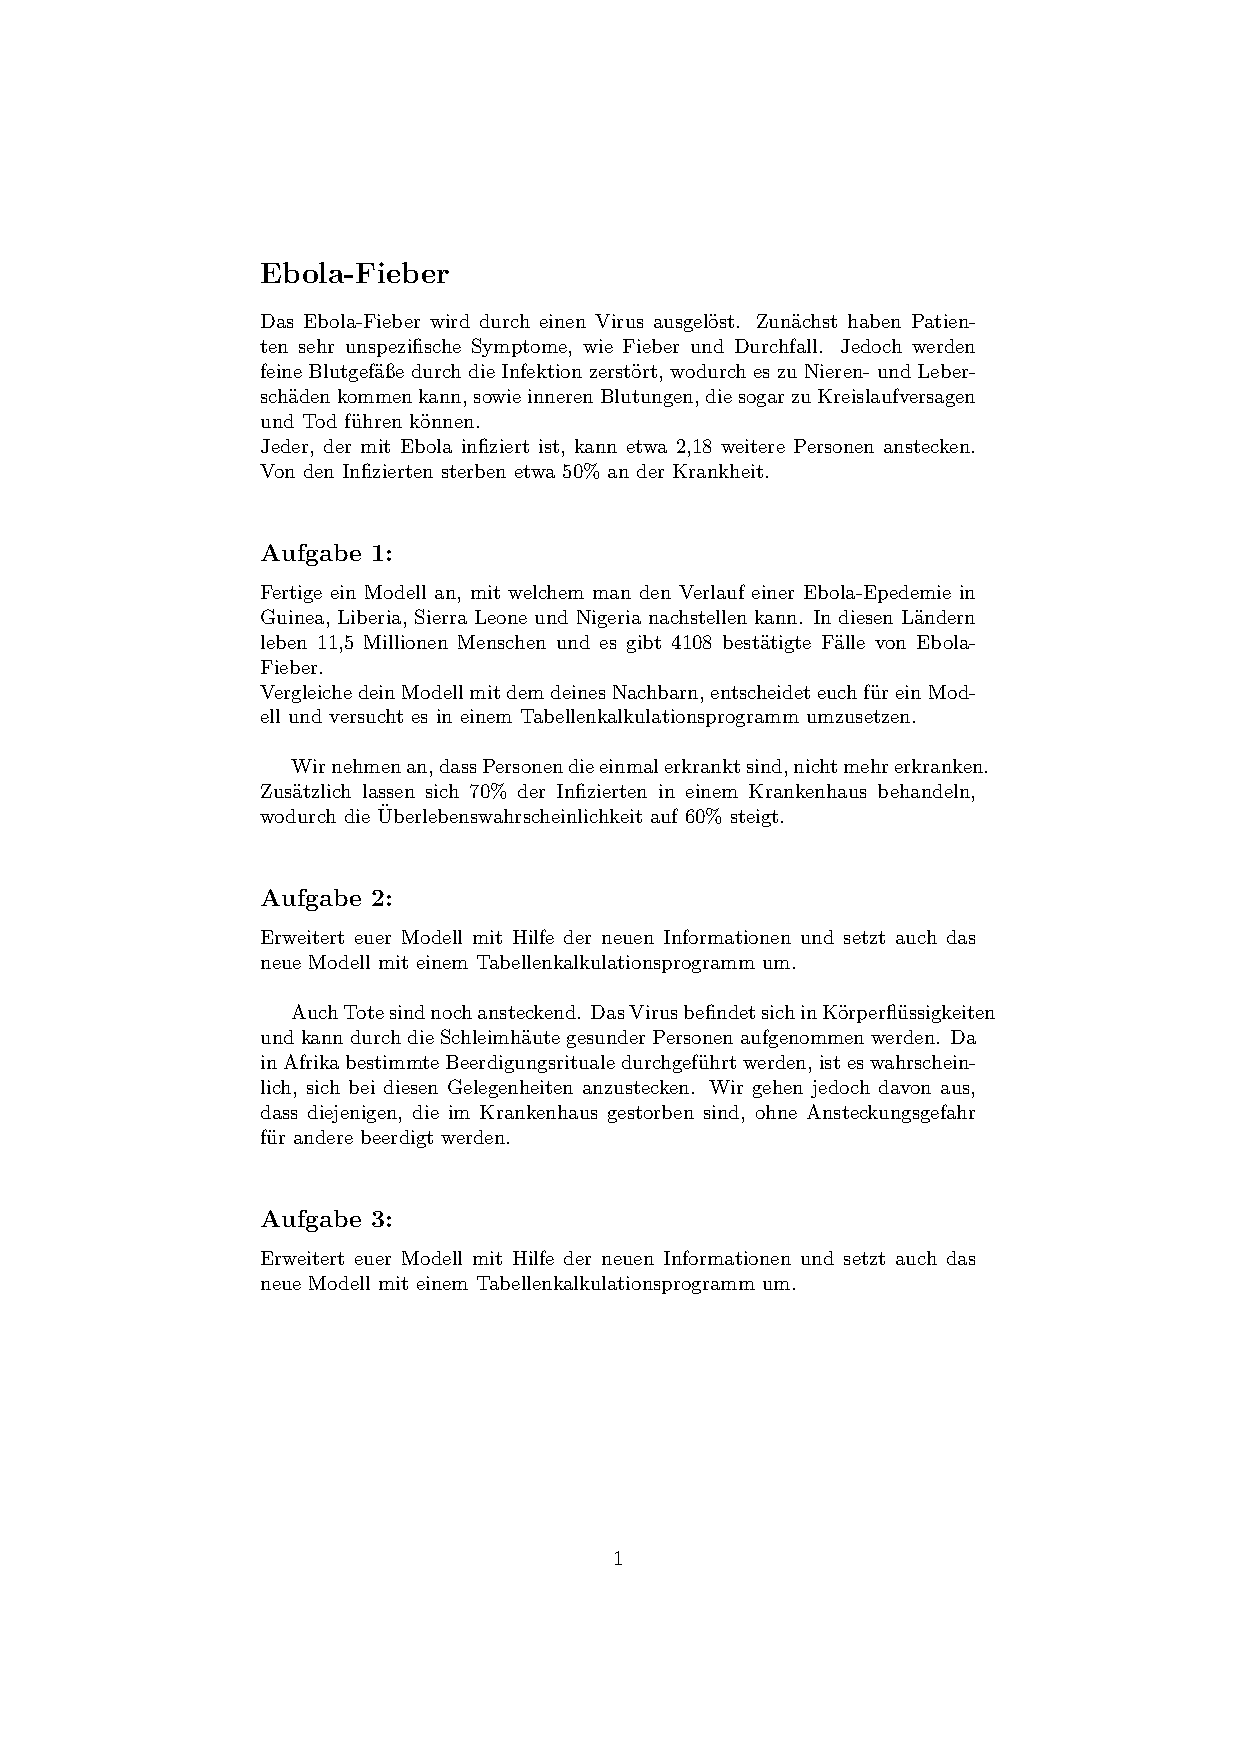
\includegraphics[width=\textwidth]{projekt/Arbeitsblatt_1}}
\subsubsection{Erwartungshorizont}
Da die Schülerinnen und Schüler bereits gelernt haben, wie sie Gleichungen aufstellen wird erwartet, dass sie zunächst einige Schritte ausprobieren und danach eine Vorschrift für eine beliebige Zeit angeben. Dies könnte dann etwa so aussehen:\\
Zunächst sollten die Kranken betrachtet werden, da diese lediglich von der Anzahl der Kranken zuvor abhängt.\\
$ K(1) = K$\\
$ K(2) = 2,18 \cdot K(1) - K(1) = 1,18 \cdot K(1)$\\
$ K(3) = 1,18 \cdot K(2) = 1,18^2 \cdot K(1)$\\
$ K(t) = 1,18^{t-1} \cdot K(1)$\\

Danach können sie eine Vorschrift für die Gesunden mit der gleichen Vorgehensweise finden.\\
$ G(1) = G$\\
$ G(2) = G(1) - 2,18 \cdot K(1) + 0,5 \cdot K(1) = G(1)- 1,68 \cdot K(1)$\\
$ G(3) = G(2) - 1,68 \cdot K(2)$\\
$ G(t) = G(t-1) - 1,68 \cdot K(t-1)$\\
Diese Gleichung kann selbstverständlich auch anders formuliert werden und explizit dargestellt werden. Diese Darstellung lässt sich jedoch leicht mit Tabellenkalkulationsprogrammen durch ziehen der Formeln umsetzen.\\

Ebenso sollen die Schülerinnen und Schüler Vorschriften für die Anzahl der Toten angeben.\\
$ T(1) = 0 $\\
$ T(t) = T(t-1) + 0,5 \cdot K(t-1)$\\


\noindent\frame{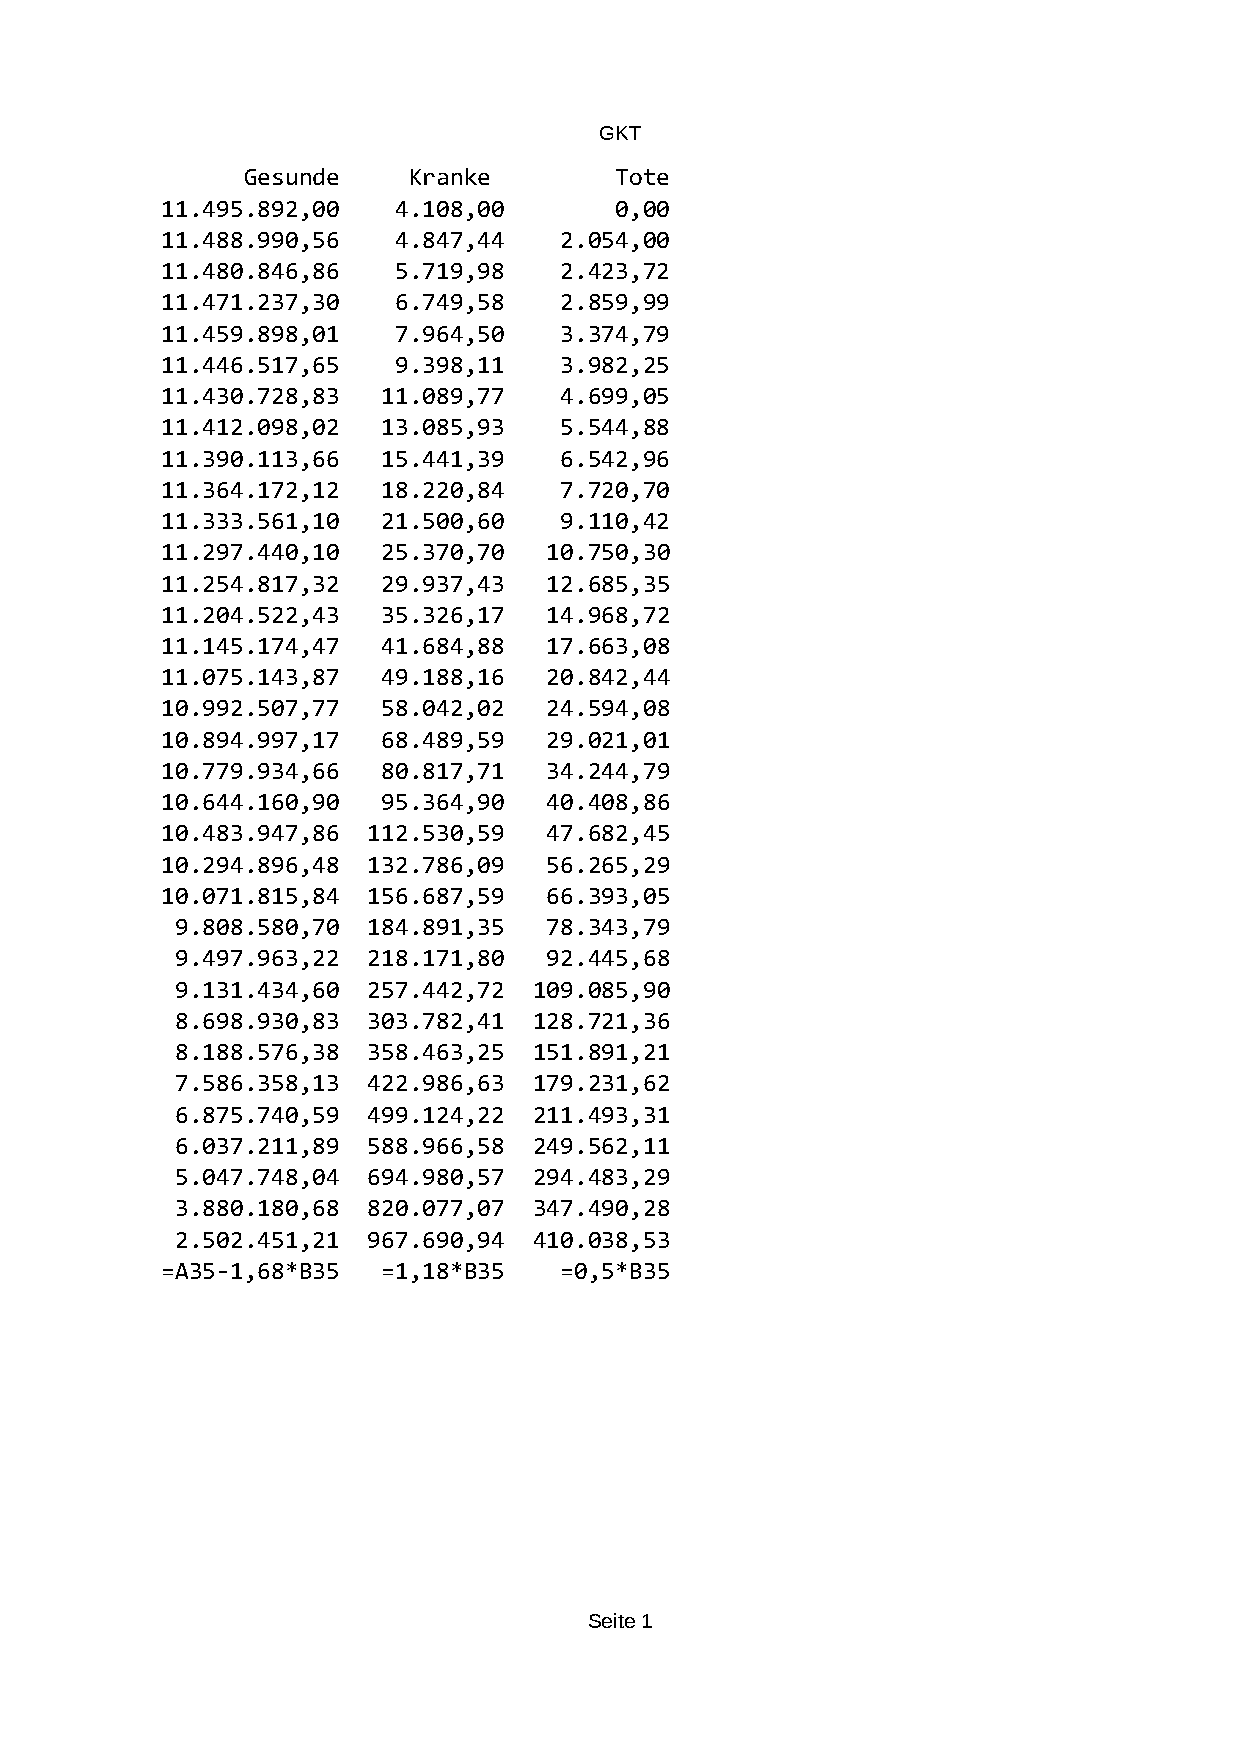
\includegraphics[width=\textwidth]{projekt/erwartung_gtk}}\newpage
\noindent\frame{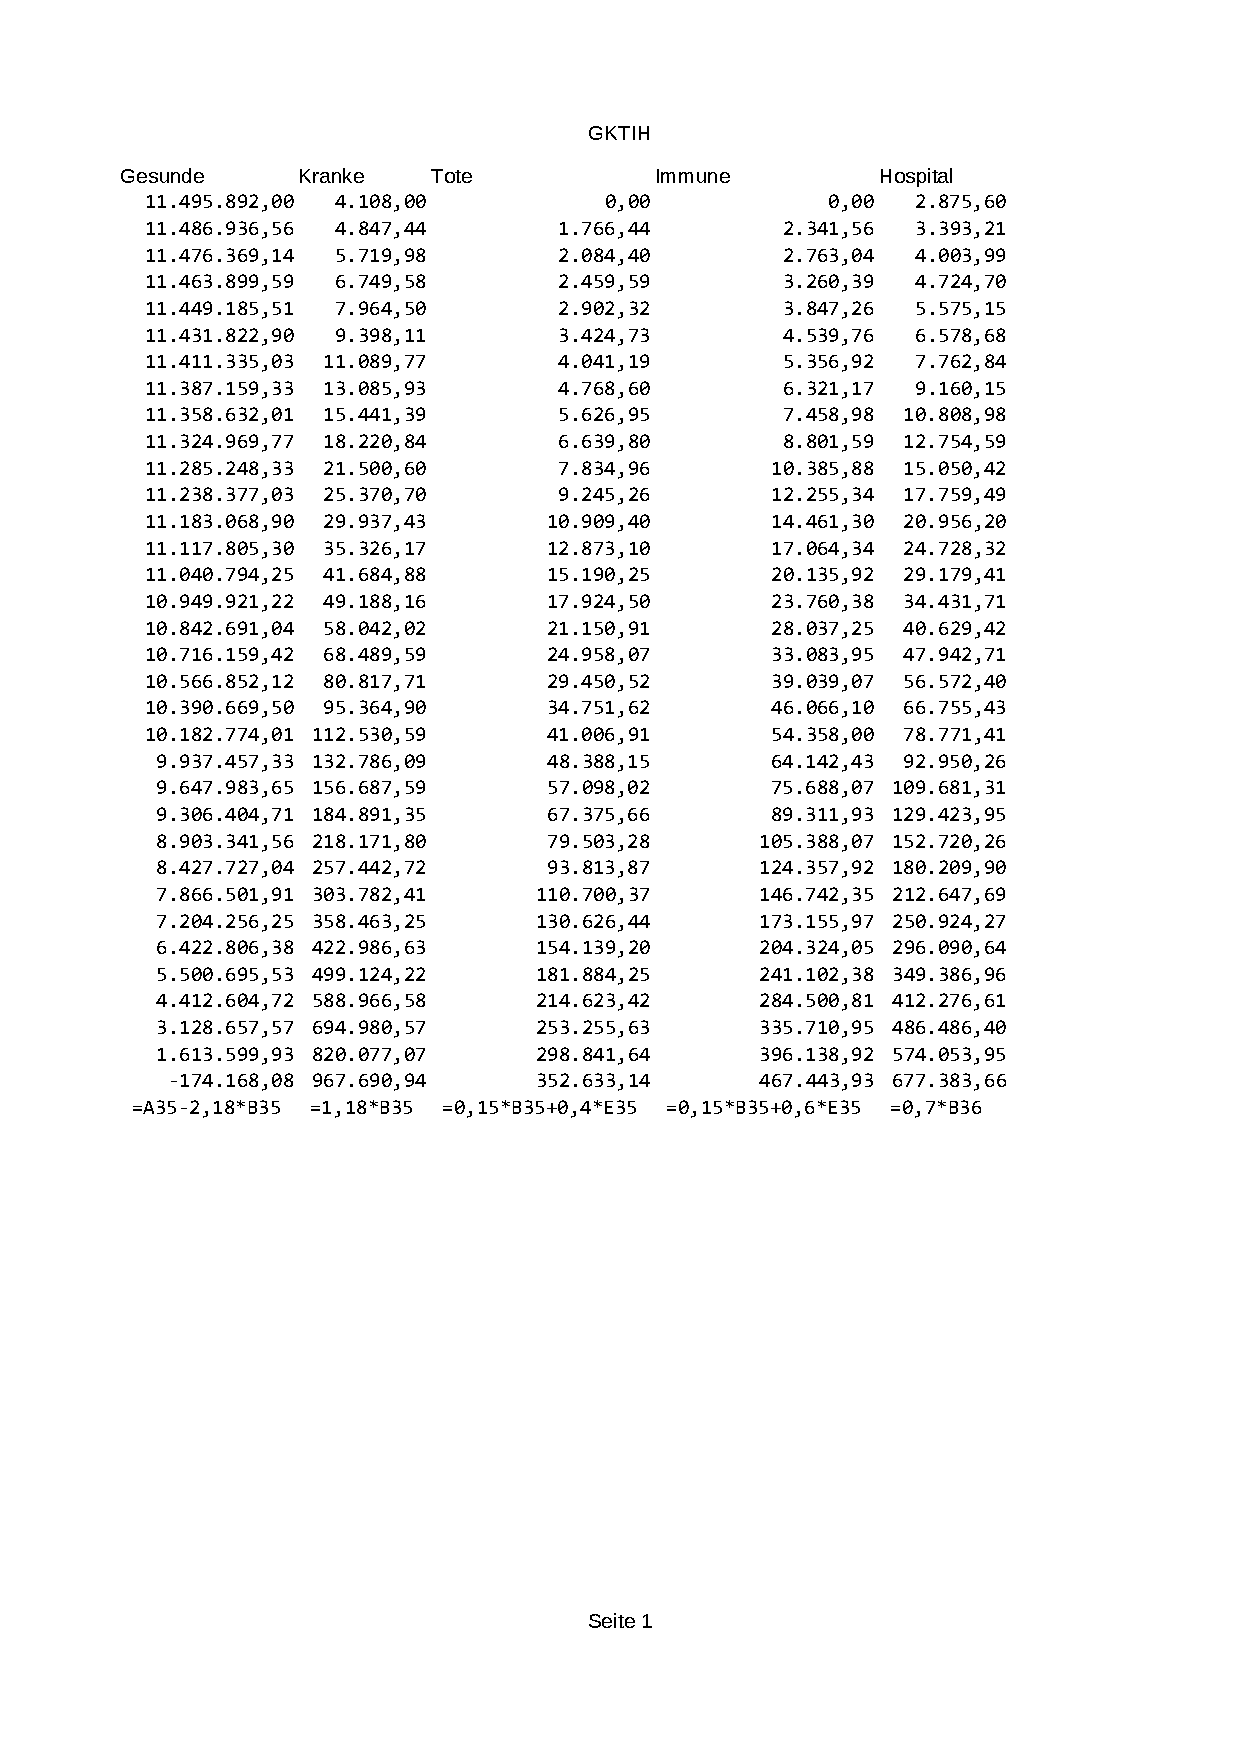
\includegraphics[width=\textwidth]{projekt/erwartung_gtih}}\newpage
\noindent\frame{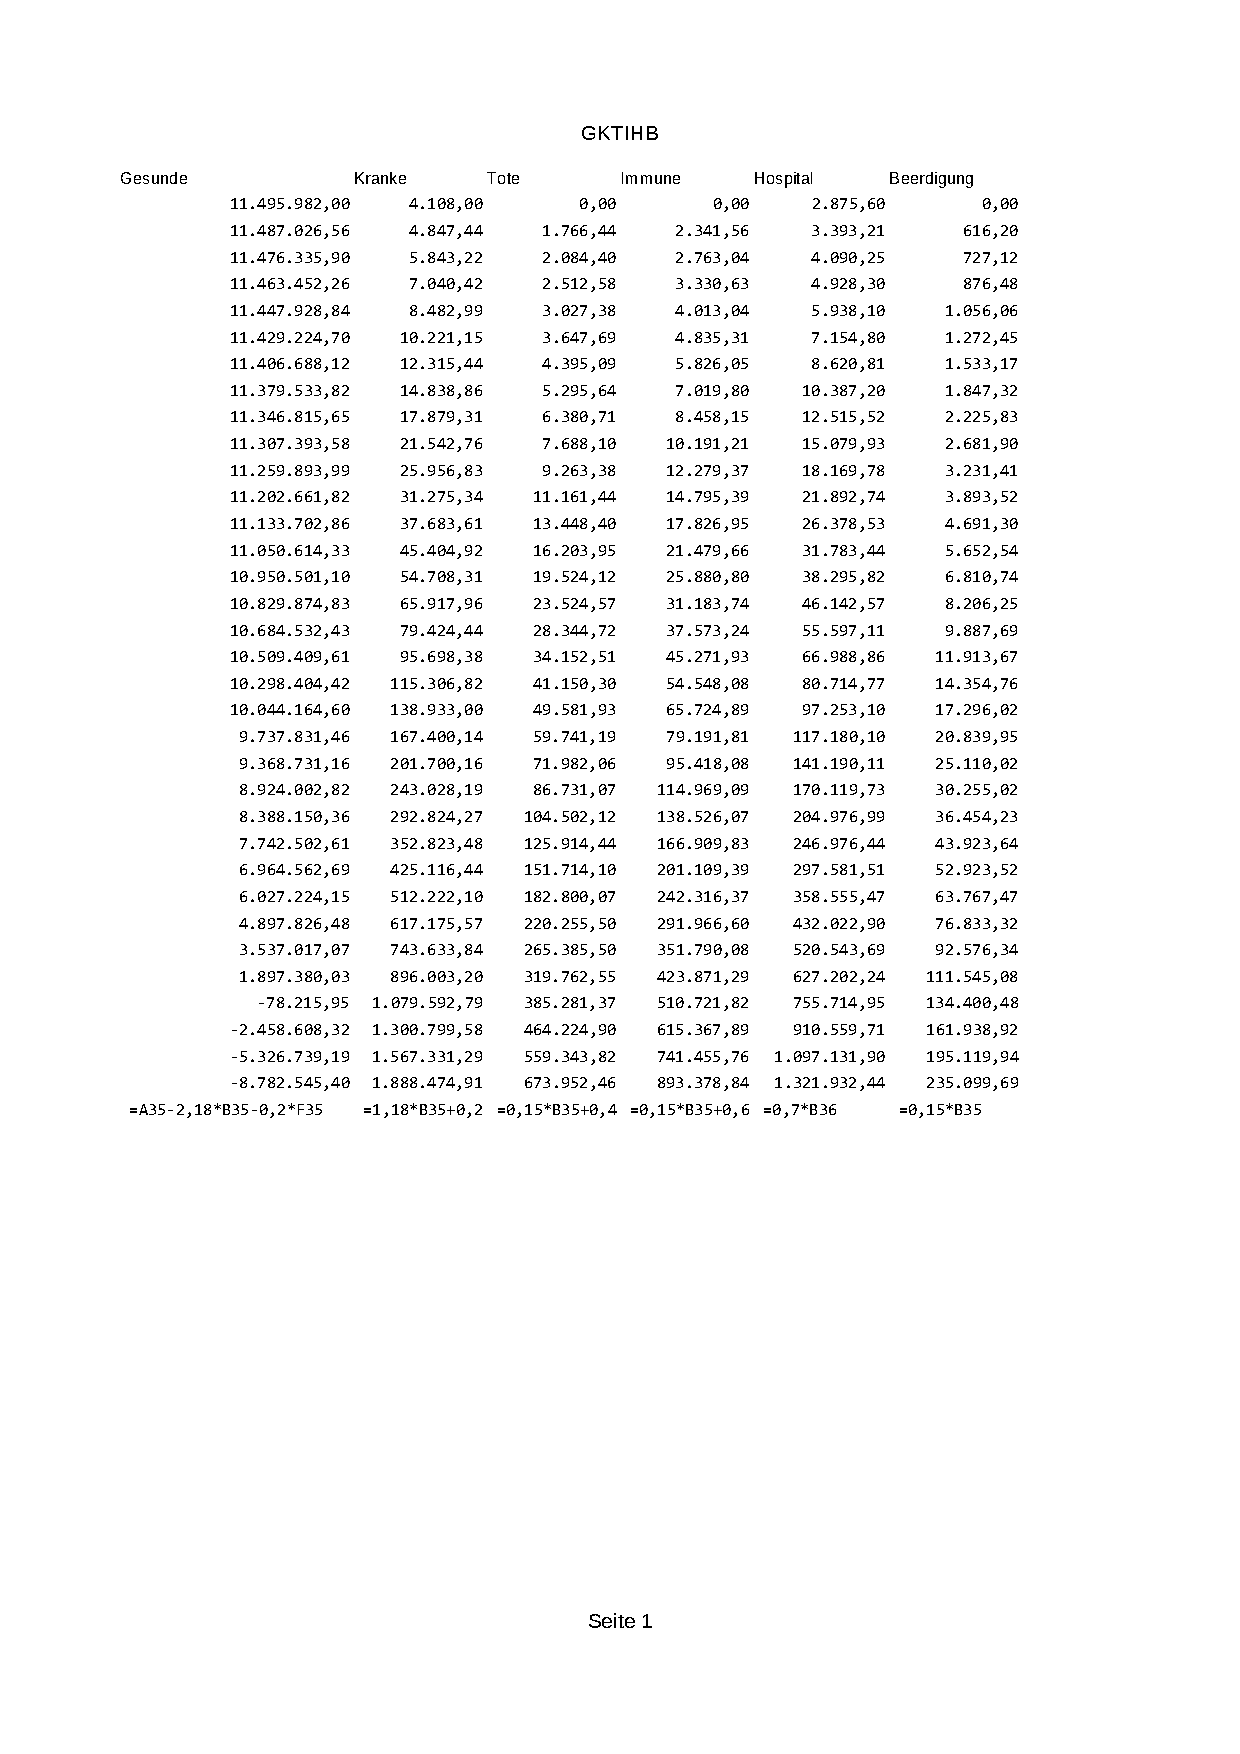
\includegraphics[width=\textwidth]{projekt/erwartung_gktihb}}\newpage
\subsubsection{Schülerprodukte}
\noindent\frame{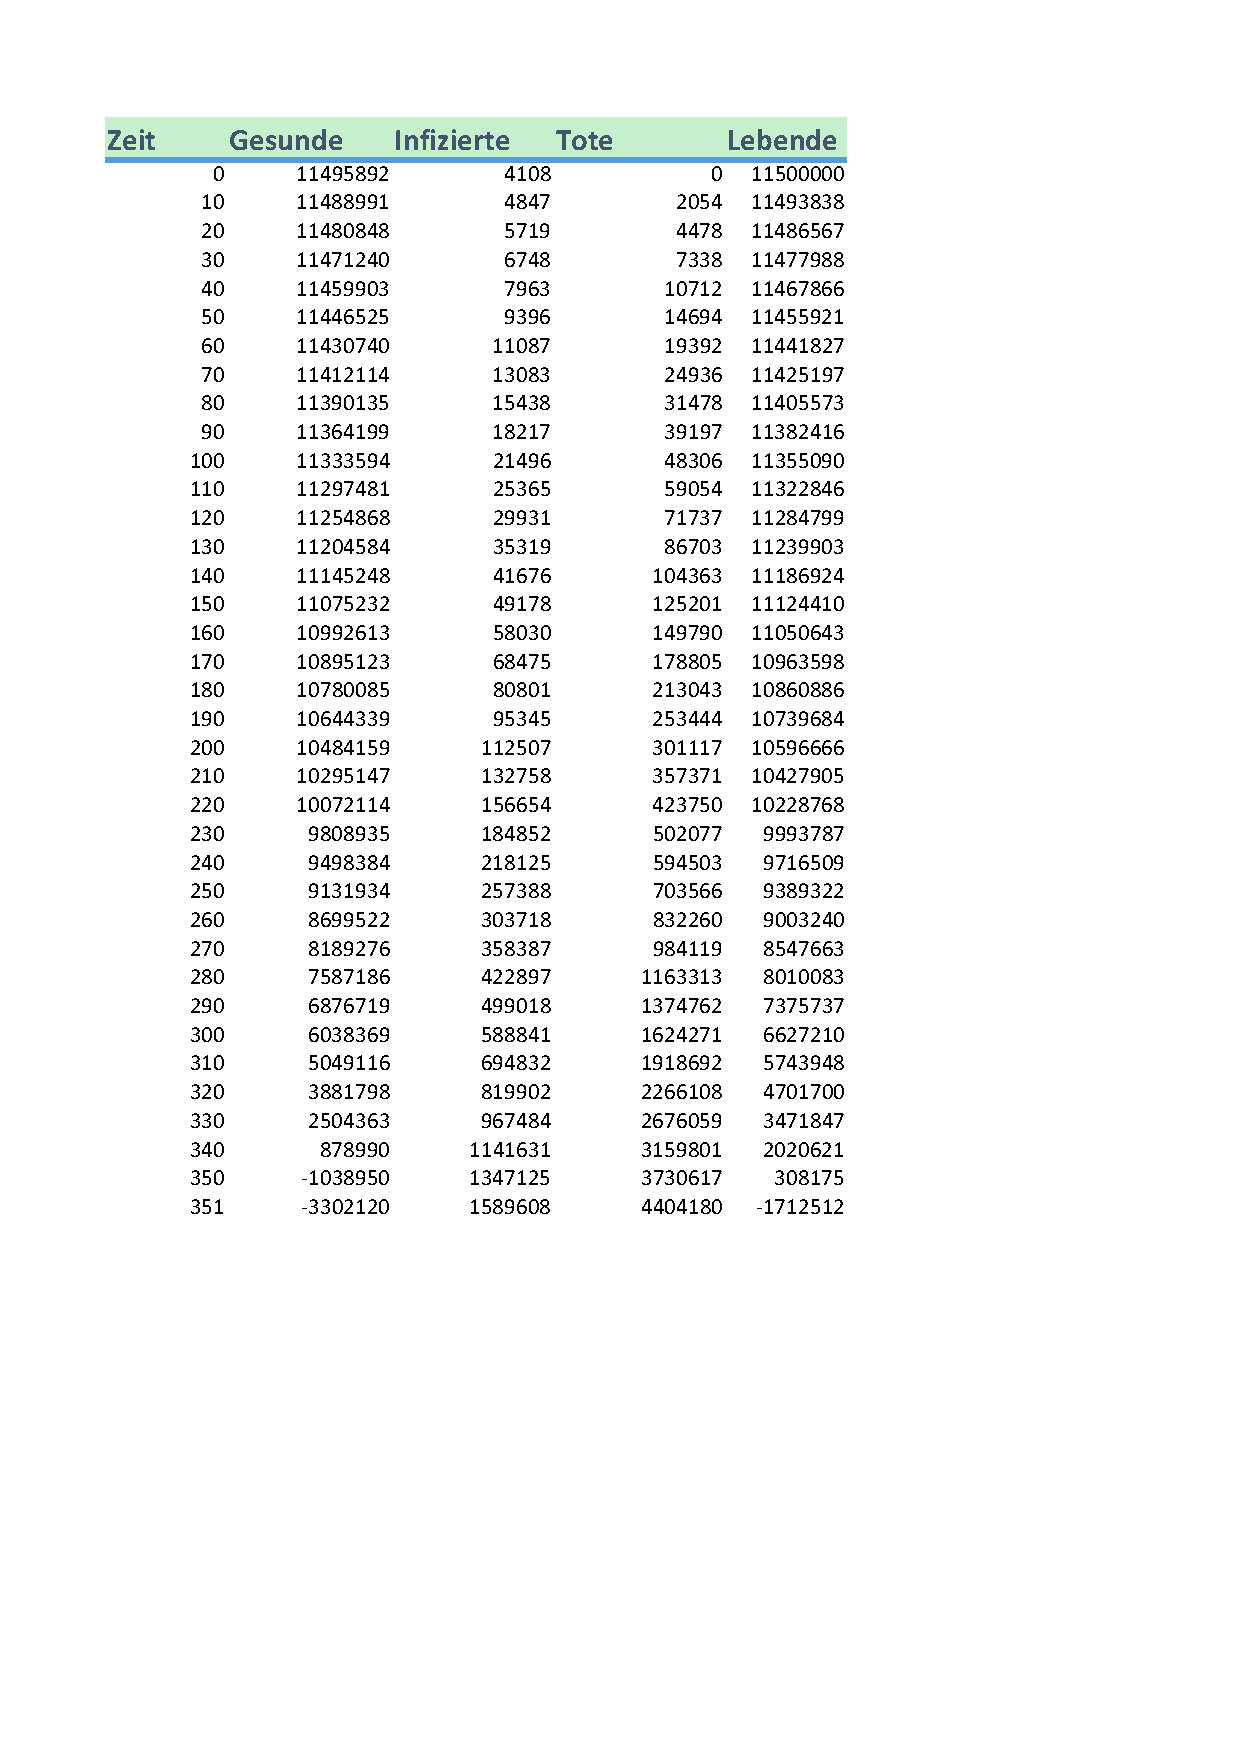
\includegraphics[width=\textwidth]{projekt/leistung_1_1}}\newpage
\noindent\frame{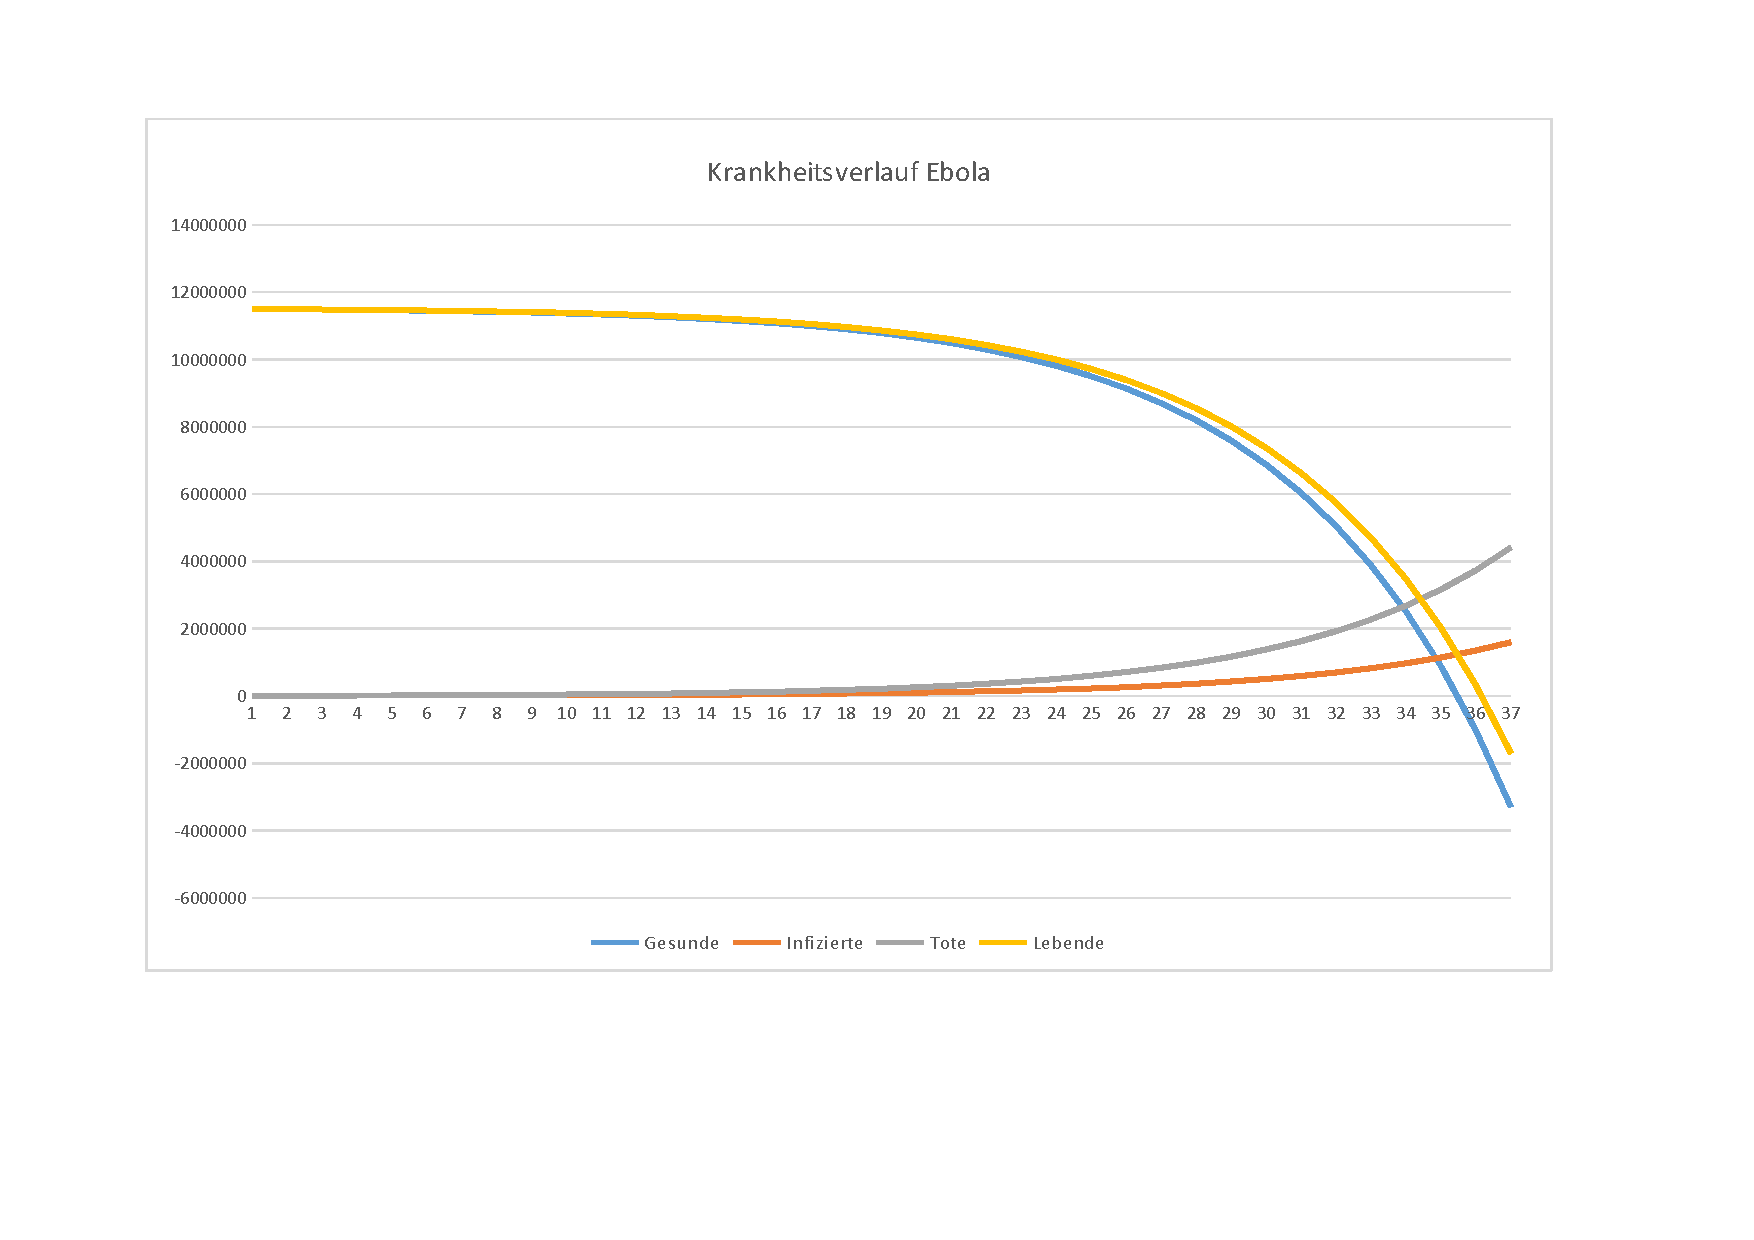
\includegraphics[width=\textwidth]{projekt/leistung_1_2}}\newpage
Alle Produkte der Schülergruppen entsprechen mindestens dem Erwartungshorizont. Das oben angeführte Beispiel zeigt aber zusätzlich ein Schülerprodukt, das die Erwartungen weit übertrifft. Darin zeigt sich, dass eine Differenzierung der Aufgabenstellungen dringend notwendig ist. Einige Gruppen benötigten viel Zeit um sich mit dem Tabellenkalkulationsprogramm vertraut zu machen, während das obige Beispiel zeigt, dass es auch Gruppen gab die nach Bearbeitung der Aufgabe noch die Zeit hatten, einen Graphen zu plotten der den Verlauf nochmal verdeutlicht.  

\subsubsection{Reflexion der Stunde}
Die Schülerinnen und Schüler haben zum Teil neue Funktionen der Tabellenkalkulationsprogramme kennen gelernt. Zudem haben sie Grundlegende Vorgänge der Modellbildung genutzt und eigenständig Modelle aufgestellt. In diesem Zusammenhang wurde auch das Aufstellen von Funktionen wiederholt und vertieft.\\
Die Schülerbeteiligung war sehr hoch, ohne Anstoß durch die Lehrperson haben sie die Vorschläge der Gruppen gemeinsam korrigiert und in einem angenehmen Klima fachlich diskutiert. Zusätzlich wurden schon früh Verbesserungsvorschläge für das Modell angebracht.\\
Da die Klasse unbekannt ist, war die Zusammensetzung in der Partnerarbeit nicht optimal. Wenn man die Lerngruppe besser kennt, könnte man Teams bilden, die sich gegenseitig unterstützen. Dadurch könnten die großen Unterschiede im Zeitbedarf angepasst werden.\\
Ist dies jedoch nicht möglich, sollte es Aufgaben geben, die die besonders schnellen zusätzlich erledigen können.\\
Statt der beiden Simulationen konnten die Gruppen in der Stunde nur eine Simulation durchführen. Dies ist jedoch von Vorteil für die nächste Sitzung, da an diesem Tag acht von siebzehn Schülern fehlten.\\
Daher wird in der nächsten Stunde eine größere Wiederholung stattfinden. Von allen Gruppen wird dann lediglich die zweite Simulation durchgeführt und die dritte Simulation steht für die besonders schnellen Schülerinnen und Schüler zur Verfügung. 
\newpage
\subsection{Projektstunde 3 \& 4}\ellen
\subsubsection{Bemerkungen zur Lerngruppe}\label{ssec:project:34:lerngruppe}
\subsubsection{Methodische Überlegungen}
\subsubsection{Verlaufsskizze}
\subsubsection{Materialien}
\subsubsection{Erwartungshorizont}
\subsubsection{Schülerprodukte}
\subsubsection{Reflexion der Stunde}
\newpage
\subsection{Projektstunde 5 \& 6}\steffen
\subsubsection{Bemerkungen zur Lerngruppe}
Ergänzend zu den Einschätzungen in Abschnitt \ref{ssec:project:34:lerngruppe} zeigt sich die Lerngruppe als durchaus motiviert. Die Schülerinnen und Schüler, die in der 1. und 2. Stunde wegen innerschulischer Aktivitäten nicht am Unterricht teilgenommen haben, gliedern sich gut in das Leistungsspektrum der Klasse ein. Es besteht weiterhin das für Informatikkurse charakteristische ``Leistungstal'' in der Mitte des Leistungsspektrums. Da es sich um eine Hochbegabtenklasse handelt, entspricht das untere Ende des Leistungsspektrums etwa einer durchschnittlichen Leistung in Regelschulen. Die Schülerinnen und Schüler sind interessiert am Kontext der Reihe, fordern aber auch Beschäftigung ein. Die Reaktion auf fragend-entwickelnden Unterricht lässt sich als zäh beschreiben. 

Das Vorwissen in der Klasse ist stark heterogen. Obwohl viele der Schüler ein Zertifikat über den Einsatz von Excel verfügen, ist der aktive Einsatz aber bei den meisten einige Jahre her. Dementsprechend muss beim Einsatz von Tabellenkalkulation entsprechend unterstützt werden. Informatische Grundbildung ist aber breit in der Klasse vorhanden. Begriffe wie ``Variable'' und ``Anweisung'' werden verstanden. 

Schüler R\footnote{Name wegen Datenschutz anonymisiert} hebt sich weiterhin von der restlichen Klasse ab im Hinblick auf die Leistung deutlich nach oben ab. Bezüglich der Sozialkompetenz zeigt sich aber Nachholbedarf. R fordert auch explizit mehr Handlungsspielräume im Unterricht.

Eine Gruppe von fünf Schülerinnen erfordert eine etwas stärkere Lehrerpräsenz während der Bearbeitung von Aufgaben, da sonst deren Aufmerksamkeit sich anderen, unterrichtsirrelevanten Themen zuwendet. 

Eine weitere Gruppe von drei Schülern benötigen ebenfalls mehr Lehrerpräsenz, da diese Gruppe zu alternativen Lösungsansätzen neigt, die jedoch in den vergangen Stunden nicht immer zu einer Lösung führt.
\subsubsection{Methodische Überlegungen}
Aus den Beobachtungen innerhalb der Vorstunde ging hervor, dass es in der Klasse noch Probleme mit der Interpretation des Netzwerkmodells gibt. Vor allem, dass die Anzahl der Individuen innerhalb des Modells konstant bleibt. Es wurde häufig beobachtet, dass die Schüler ausgehende Kanten nicht beachten. Da dieses Verständnis aber essentiell für den weiteren Verlauf der Reihe ist, muss hier entsprechend korrigierend gewirkt werden. Eine Möglichkeit wäre es, dies mit einem Lehrvortrag zu tun, in dem diese Zusammenhänge explizit erklärt werden. Die Lerngruppe neigt aber dazu, bei Vorträgen sehr schnell das Interesse und damit auch die Aufmerksamkeit zu verlieren. Aus diesem Grund sollte auf Vorträge in dieser Klasse verzichtet werden. Organischer und Schülerzentrierter ist dagegen der folgende Ansatz: Den Schülern wird das Netzwerksmodell präsentiert. Anschließend sollen sie zuerst den Weg eines Individuums durch den Graph beschreiben. Anschließend werden die Iterationsvorschriften in nicht-zusammengefasster Form präsentiert. Die Schüler sollen sich nun gegenseitig mittels \emph{Think-Pair-Share} die Vorschrift für $K(n)$ erklären. 

Nachdem das Modell für alle einheitlich festgesetzt wurde, sollen nun Maßnahmen zur Eindämmung einer Krankheit modelliert werden. Der bisherige Ansatz wurde von der Klasse als zu kleinschrittig empfunden. Um weiterhin die Motivation der Klasse zu erhalten, wird der Arbeitsauftrag wesentlich freier als bisher gestaltet. Informationen, die die Schüler in eine gewisse Richtung führen sollen, werden nicht gegeben. Der Auftrag beinhaltet die Modellierung der Maßnahmen sowie deren Integration in das bestehende Modell und der Auswertung mit Excel. Gefordert werden mindestens zwei Maßnahmen. Durch die Formulierung ``mindestens'' können die Leistungsspitzen in der Klasse abgefangen werden. Um schwächere Schüler nicht zu verlieren, wird der Auftrag als Gruppenarbeit gegeben. Eine Bearbeitung mit maximal drei Schülern erachte ich als praktikabel. Alternativ ließen sich die Maßnahmen auch fragend-entwickelnd modellieren. Die Lerngruppe scheint aber noch nicht genug mit einem schülerzentrierten Unterricht vertraut zu sein, um die Maßnahmen in einer Unterrichtsdiskussion flüssig erarbeiten zu können. Die Diskussion liefe Gefahr zu lehrerzentriert zu werden und nur kleine Teile der Lerngruppe zu aktivieren. Der gruppenbasierte Ansatz ist darum vorzuziehen.

Die Evaluation der Ergebnisse soll ebenfalls schülerzentriert erfolgen. Ziel ist es, dass die Schüler ihre Ergebnisse sich gegenseitig präsentieren und miteinander besprechen und gegebenenfalls verbessern. Um Redundanzen zu vermeiden, werden zuerst die Ansätze im Plenum gesammelt. Dazu dient die Tafel beziehungsweise das Smartboard. Gesammelt werden nur die Maßnahmen selbst. Modellierungen werden erst danach in das bestehende Modell eingeführt. Nachdem ein Maßnahmenkatalog erstellt wurde, können die verschiedenen Modellierungen in der Klasse diskutiert werden. Gruppen, die eine Maßnahme modelliert haben, fügen diese in das bestehende Modell ein und erläutern ihre Modellierung. Der Rest der Klasse wird dazu aufgefordert, Anmerkungen und Verbesserungen beizusteuern, falls nötig. Bei Gruppen, die ihre Maßnahme in ihre Tabellenkalkulation eingebunden haben, kann zudem auf die Effektivität der Maßnahme eingegangen werden. 

Aufgrund bereits geäußerter Ideen der Schüler, kann mit der Maßnahme ``Auswandern'' gerechnet werden. Falls diese Maßnahme nicht von der Klasse modelliert wurde, muss sie als Impuls vom Lehrer kommen. Dazu kann ``Gerade im Falle von Ebola, wo die Letalität bei 50$\%$ liegt, würde Ich nicht auf eine Impfung warten wollen. Welche Optionen hätte ich denn sonst noch?''. Die Nennung einer Maßnahme hängt natürlich von den zuvor modellierten Schülermaßnahmen ab. Ziel ist es, von der Betrachtung einer einzelnen Population hin zur Betrachtung mehrerer zu kommen. Den Schülern sollte implizit klar sein, dass bisher immer der Krankheitsverlauf innerhalb eines Landes betrachtet wurde, da dies auch so eingeführt wurde.

Mit der Erwähnung von vier Fällen von Ebola, die im Herbst 2014 in den USA entdeckt wurden, sollen die Schüler erkennen, dass das bisherige Modell einen Krankheitszustand noch nicht integriert hat, nämlich die Klasse der Inkubierenden, die es erlaubt, eine Krankheit über Grenzen hinweg zu tragen. Diese soll von den Schülern in das bestehende Modell eingebunden werden. Dazu wäre die bisher verwendete Partnermodellierung geeignet. Die Einbindung sollte aber keinen der Schüler vor ein Problem stellen, weswegen dieser Schritt zeitsparender in einem Lerngruppengespräch absolviert werden kann. Eine direkte Einführung, in der der Lehrer der Lerngruppe die Klasse der Inkubierenden vorstellt und selbst einbindet, sollte vermieden werden. Diese Krankheitsklasse ist ein wichtiges Element in der Modellierung von Pandemien und sollte darum auch von der Lerngruppe selbst erkannt und modelliert werden. 

Nachdem das Modell einer einzelnen Population fertig gestellt ist, werden nun die Interaktionen zwischen verschieden Populationen modelliert. Wieder soll den Schülern genügend Freiheiten gelassen werden, um eigene Ideen umsetzen zu können. Gleichzeitig muss gerade jetzt von Seiten der Lehrperson Kontrolle ausgeübt werden, damit die Schüler sich nicht in Details oder Komplexität verlieren. Ziel ist es, am Ende der Stunde ein verwendbares Modell für die Simulation von Pandemien zu haben. 

Die Modellierung der Interaktionen wird wieder in Gruppenarbeit von den Schülern selbst durchgeführt. Als Orientierungshilfe dient die Anweisung, Faktoren zu beschreiben, die den Individuumsaustausch zwischen zwei Populationen beeinflussen. Diese Faktoren sollen dann mit Werten aus $[0,1]$ quantifiziert werden. Durch die Vorgabe der Modellierung erhalten schwächere Schüler einen klar abgesteckten Handlungsrahmen, während stärkere Schüler immer noch genügend eigene Ideen einbringen können. 

Die Evaluation der Ergebnisse erfolgt, wie schon zuvor, mit einer vorgelagerten Sammlung von Lösungen. Die Schüler werden danach wieder ermutigt, ihr Modellierungen vor der Klasse zu beschreiben. Redundanzen und stark verwandte Faktoren werden dabei zusammengefasst. Der Impuls dazu sollte von der Lerngruppe selbst kommen, kann aber zur Not auch vom Lehrer eingebracht werden. Diese Evaluation bietet sich auch als mögliches Stundenende an. 

Sollte die Lerngruppe schneller als erwartet die Aufträge erledigen und evaluieren, dient als Stundenpuffer die Implementierung des erarbeiteten Modells für zwei Populationen in einer Tabellenkalkulation. Besonderheit soll dabei sein, dass es diesmal einen ``Patienten 0'' gibt, von dem die Krankheit ausgeht. Dieser Anwendungsfall dürfte Interesse in der Klasse wecken, zumal bisher immer nur der Verlauf einer bereits ausgebrochenen Krankheit simuliert wurde. Aufgrund der komplexen Iterationsvorschriften, die sich durch die zweite Population ergeben, wird nicht erwartet, dass alle Schüler diese Aufgabe noch in dieser Stunde fertig stellen. Schüler denen dies doch gelingt, werden aufgefordert, ihren Klassenkameraden zu helfen. Ziel des Auftrages ist es, die Schüler erkennen zu lassen, dass eine Tabellenkalkulation nicht mehr die beste Wahl für eine Simulation des erarbeiteten Modells ist. Die Motivation der Aufgabe erwächst aus dem Modellierungskreislauf. Die Frage, ob die simulierten Werte adäquat die Wirklichkeit beschreiben und welche Schwächen das Modell noch hat, werden auf die nachfolgende Stunde verschoben.

Die obige Planung bezieht sich auf die Situation, dass eine 7. und 8. Stunde mit der Klasse zur Verfügung stehen. Für den Fall, dass diese Doppelstunde die letzte in dieser Reihe ist, muss die zweite Hälfte der Stunde um geplant werden, um das Reihenziel, die Durchführung des Modellierungskreislaufs, zu erreichen. Auf die Modellierung von mehreren Populationen wird verzichtet und stattdessen wird die Simulation und Evaluation des Modells behandelt. Damit werden die bisher unterrepräsentierten Teile des Modellierungskreislaufs in den Vordergrund gerückt.

In diesem Fall werden der bereits geplante Stundeneinstieg übernommen. Der erste Auftrag wird ebenfalls übernommen, jedoch ohne die Puffer-Aufgabe. Als Puffer dient die absichtlich offen gehaltene Anzahl an zu modellierenden Maßnahmen. Auch die Planung der Evaluation der Ergebnisse bleibt unverändert. 

Um den Bezug zur Reihe aufrecht zu erhalten, wird der Modellierungskreislauf noch einmal besprochen. Ziel ist es, den Schülern den Weg aufzuzeigen, den sie bisher im Modellierungskreislauf genommen haben und die nächsten Schritte zu planen. Ein Lehrervortrag kann an dieser Stelle Zeit sparen, während eine schülerzentrierte Diskussion das selbstbestimmte Lernen der Schüler fördert. Da die Klasse meiner Meinung nach noch nicht viel Kontakt mit schülerzentriertem Unterricht hatte, entscheide ich mich für den letzteren Ansatz. Es wird erwartet, dass die Schüler als nächsten Schritt das Simulieren eines Krankheitsverlaufs identifizieren werden. 

Dementsprechend soll im nächsten Schritt das erstellte Modell und die Maßnahmen an einem Fallbeispiel untersucht werden. Die Schüler erhalten als Aufgabe, ihre bereits vorhandene Tabellenkalkulation ab Zeitschritt $10$ entsprechend anzupassen. Die Aufgabe ist bewusst offen formuliert. Die Schüler können sich entscheiden, die eigenen Ergebnisse oder die anderer Gruppen umzusetzen. Als Fallbeispiel dient der Ebola-Ausbruch in Sierra Leone in 2014. Da die Klasse sich bisher als vergleichsweise leistungsstark präsentiert hat, wird von zu viel Restriktion in der Ausgestaltung der Aufgabe abgesehen. 

Bei der Evaluation sollen im Idealfall alle Gruppen ihre Ergebnisse präsentieren. Dopplungen sind hier eher unwahrscheinlich, da jede Gruppe andere Maßnahmen implementiert. Bei der Präsentation soll vor allem immer die Frage ``Haben die Maßnahmen Wirkung gezeigt?'' im Vordergrund stehen. Dadurch wird der Sinn und Kontext des Auftrags betont. Die Klasse wird zudem aufgefordert, die Ergebnisse zu diskutieren und deren Plausibilität zu bewerten. 

Am Ende der Stunde steht, dem Modellierungskreislauf folgend, die Evaluation der Simulationsergebnisse mit den realen Daten. Diese werden massiv von den Schülerergebnissen abweichen. Wichtig ist, dies nicht unkommentiert im Raum stehen zu lassen, sondern mit den Schülern zu diskutieren, wo der Unterschied herkommt und wie man in weiteren Iterationen das Modell verbessern könnte. Ein Lehrervortrag wäre an dieser Stelle unangebracht, da sich die Stunde dem Ende neigt und die Aufmerksamkeit der Schüler am Unterricht tendenziell schwerer aufrecht zu erhalten ist. 

Den Abschluss bildet eine Feedback-Runde zur gesamten Reihe. Damit die Schüler, die noch nicht so sehr mit dem Prinzip des konstruktiven Feedbacks vertraut zu sein scheinen, ihre Meinung auch offen wiedergeben können, wird das Feedback nicht mündlich sondern anonymisiert und schriftlich erfolgen. 

\begin{landscape}
\subsubsection{Verlaufsskizze Version 1}
\noindent
\begin{longtable}{|C{0.3\textwidth}|L{0.8\textwidth}|L{0.4\textwidth}|}
\hline
Phase & Arbeitsauftrag & Sozialform\\
\hline\hline
\endhead
\hline
\endfoot
Einstieg& Wdh: Zustandsmodell \& Iterationsvorschriften. ``Ein Individuum namens Alice ist gesund. Beschreibe anhand des Modells, was mit Alice in den nächsten Tagen passiert''

Anschließend:``Wieso sieht $K(n)$ so aus?'' in TPS& Unterrichtsgespräch\\\hline
Auftragsübergabe&``Welche Möglichkeiten gibt es, die Ausbreitung einer Krankheit zu verhindern oder zu verlangsamen? Modelliert mindestens 2 Maßnahmen und integriert diese in das bestehende Modell.''

Puffer: ``Integriert die Maßnahmen in Euer TK-Sheet''&\\\hline
Erarbeitung&Zeitansatz $\approx$ 20min&Einzel- oder Partnerarbeit\\\hline
Evaluation&Schüler präsentieren Ihre Ergebnisse. Bei Schülern, die die Zusatzaufgabe erfüllt haben, wird zudem gefragt ``Wie haben sich die Maßnahmen auf den Krankheitsverlauf ausgewirkt''&Schülerpräsentation \& Diskussion\\\hline
Auftragsübergabe&``Im Herbst 2014 gab es 4 Fälle von Ebola in den USA. Die Betroffenen waren allesamt Helfer während der Ebola-Epidemie in Afrika. Wie kam es dazu, wenn Flugzeuge keine offensichtlich kranken Passagiere befördern? Wie muss das Modell ergänzt werden?''&\\\hline
Erarbeitung&$\approx$ 5min&Unterrichtsgespräch\\\hline
Auftragsübergabe&``Modelliert die Interaktion zwischen zwei Populationen. Identifiziert dazu Einflussfaktoren, wegen denen Menschen von einer Population in eine andere wechseln. Beschreibt jeden Einflussfaktor mathematisch als Zahl in $[0,1]$''&\\\hline
Erarbeitung&$\approx$ 15min&Einzel-/Gruppenarbeit\\\hline
Evaluation&Einflussfaktoren werden gesammelt und anschließend von den Schülern präsentiert.&Schülerpräsentation \& Diskussion\\\hline\hline
&Mögliches Stundenende&\\\hline\hline
Auftragsübergabe&``Erzeugt eine TK, mit der die Interaktion zwischen zwei modellierten Populationen beschrieben wird. Die Simulation beginnt dieses mal mit nur einem Infizierten in einer der beiden Populationen''&\\\hline
Erarbeitung&Bis Stundenende&Einzel-/Gruppenarbeit\\
\end{longtable}

\end{landscape}
\begin{landscape}
\subsubsection{Verlaufsskizze Version 2 (durchgeführt)}
\noindent
\begin{longtable}{|C{0.3\textwidth}|L{0.8\textwidth}|L{0.4\textwidth}|}
\hline
Phase & Arbeitsauftrag & Sozialform\\
\hline\hline
\endhead
Einstieg& Wdh: Zustandsmodell \& Iterationsvorschriften. ``Ein Individuum namens Alice ist gesund. Beschreibe anhand des Modells, was mit Alice in den nächsten Tagen passiert''

Anschließend:``Wieso sieht $K(n)$ so aus?'' in TPS& Unterrichtsgespräch\\\hline
Auftragsübergabe&``Welche Möglichkeiten gibt es, die Ausbreitung einer Krankheit zu verhindern oder zu verlangsamen? Modelliert mindestens 2 Maßnahmen und integriert diese in das bestehende Modell.''&\\\hline
Erarbeitung&Zeitansatz $\approx$ 15min&Einzel- oder Partnerarbeit\\\hline
Evaluation&Schüler präsentieren Ihre Ergebnisse&Schülerpräsentation \& Diskussion\\\hline
Reflexion&``Welche Teile des Modellierungskreislaufs haben wir schon abgearbeitet, welche fehlen noch?''&Schülergespräch\\\hline
Auftragsübergabe&``Es sollen nun Vorhersagen mit eurem Modell getroffen werden. Implementiert dafür das Modell für Sierra Leone ($7\cdot 10^6$ Einwohner, $15$ Infizierte zu beginn). Implementiert ab $n=10$ zwei Maßnahmen. Wie wirken sich die Maßnahmen aus?''&\\\hline
Erarbeitung&Zeitansatz $\approx$ 20min&Einzel-/Gruppenarbeit\\\hline
Evaluation&Schülergruppen präsentieren ihre Ergebnisse. Da die Auswahl der zu implementierenden Maßnahmen frei ist, sind verschiedene Kombinationen zu erwarten. Mehrere Gruppen präsentieren&Schülerpräsentation\\\hline
Reflexion&``Vergleichen wir das mit realen Daten. Was fällt auf? Bildet das Modell die Wirklichkeit gut genug ab?'' und anschließend ``Woher kommen die Unterschiede. Wie könnte man das Modell verbessern?''&Diskussion\\\hline
Abschluss&Ausblick auf Weiterführendes und allgemeines Feedback der Klasse zur Reihe&Feedbackrunde\\\hline
\end{longtable}
\end{landscape}

\subsubsection{Materialien}
\subsubsection{Erwartungshorizont}
\subsubsection{Schülerprodukte}
\subsubsection{Reflexion der Stunde}
Meines Erachtens nach haben die meisten Schüler die Lernziele erreicht. Die Schüler konnten das Modell der Vorstunde erklären und Maßnahmen zur Eindämmung modellieren. Ebenso sind die verschiedenen Stadien des Modellierungskreislaufs von den Schülern verstanden und durchlaufen worden. Ausnahme bildeten 2 Schüler, die heute generell wenig Motivation zeigten. 

Ich bin der Mitarbeit der Klasse sehr zufrieden. Die Beteiligung an Fragen und Diskussionen war hoch und bisher eher ruhige Schülerinnen und Schüler haben sich eingebracht. Das handlungsorientierte Stundenkonzept wurde von der Klasse erneut gut angenommen. Die Ergebnisse, sofern vorhanden, entsprachen meinen Erwartungen an die Klasse.

Weniger zufrieden bin ich mit meiner Handhabung der weniger motivierten Schüler. Meine Versuche, die Schüler doch zur Mitarbeit zu motivieren, zeigten unterm Strich nur bei 2 von 4 Wirkung. Ein ähnlich gelagertes Problem hatte ich mit einer anderen Gruppe, die zwar motiviert mitgearbeitet, aber sich zu sehr in Details verloren hat, wodurch sie am Ende der Bearbeitungszeit des zweiten Auftrags kein fertiges Produkt vorweisen konnte. An dieser Stelle hätte ich müssen das Problem früher erkennen und entsprechend gegensteuern. Bezüglich des Vorwissens, wurde die Erfahrung der Schüler mit Excel von mir falsch eingeschätzt. Zwei Schüler hatten massive Probleme mit der Handhabung, wodurch sich in diesen beiden Fällen die oben beschriebene Demotivation erklären lässt. Die Aufwandseinschätzung des zweiten Arbeitsauftrages deckte sich nicht mit der tatsächlichen Leistung der Klasse, die meisten Gruppen haben nach 15 Minuten zusätzlicher Zeit keine verwertbaren Ergebnisse gehabt. Eine Neukonzeption der Aufgabe wäre folglich angebracht. Gleichzeitig fehlte eine Pufferaufgabe für die beiden Gruppen, die in der veranschlagten Zeit präsentierbare Ergebnisse generieren konnten. Weiterhin wurde meine Körperhaltung stellenweise als ablehnend empfunden. 

In Zukunft würde ich den Stundenaufbau im Prinzip beibehalten. Es muss aber eine bessere Analyse der Lerngruppe und deren Vorwissens erfolgen, um die Machbarkeit und den Aufwand der einzelnen Aufträge besser abschätzen zu können. Eine Reduktion der Gestaltungsfreiheit liegt auf Grund der Probleme im zweiten Auftrag nahe. Der Arbeitsauftrag könnte in kleinere Schritte aufgeteilt werden oder die Evaluation vom ersten Auftrag verbindlich für alle Gruppen festgehalten werden. Zudem muss ich an meiner Körpersprache und dem Klassenmanagement noch arbeiten. 
\subsubsection{Feedback der Schüler}